\chapter{Results}
Simulating real applications in virtual hardware without any real interaction is hard and there are many things that can break along the way. The simulations were run on a by Chalmers provided compute cluster and took quite some time to complete. This cluster luckily used an older version of Ubuntu with a relatively old kernel, and since PIN 2 depends on older kernel functionality it meant it could be run without a hitch. In addition, in order to support the old ABI used with some of its binaries while having full support for C++11, GCC 4.9.4 had to be used, specifically. 
\bigskip

TODO: In this chapter we will first measure what latency behaviour looks like when using one single HMC device, with a single link hop. Then we will increase the number of devices and always use the device at the end of the chain, e.g. when having 8 devices we will perform all allocations on the 8th device. We will view these results both from a device and a application perspective. Finally, we present a short summary of our findings.

\section{Simulation}
The simulations were run with multiple configurations, where every application (stated in \ref{method-benches}) was run with either 4 or 8 links configured, enabling between 1 and 6 memory cubes and data was allocated on the last memory unit in the network. The reason for testing both 4 and 8 links was to see whether the increased bandwidth, and in this case amount of parallelism, would significantly impact the latencies. Time of flight is measured from the memory controller's point of view, i.e., from when it was first sent from the host to when the response arrived back. 
\bigskip

The first application to be run is the, arguably, most memory intensive and latency sensitive benchmark in the SPEC2006 suite - 429.mcf. The graph \ref{Memory-access-429-single}, visualising access times when a single HMC device is being used, shows that there is a lot of latency going on during application run time, even though the only contention available is from its own memory requests. Additionally, there are notable peeks present at precisely 93 ns intervals. This could be explained as pointer chasing, where first hit is pointer lookup and the second hit, i.e. 93 ns later, is the data lookup. Between the peaks the latency patterns look quite similar. Having just one memory device is the most efficient solution available in this situation, hence we denote this as an optimal solution.
\bigskip

\begin{figure}[!h]
    \centering
    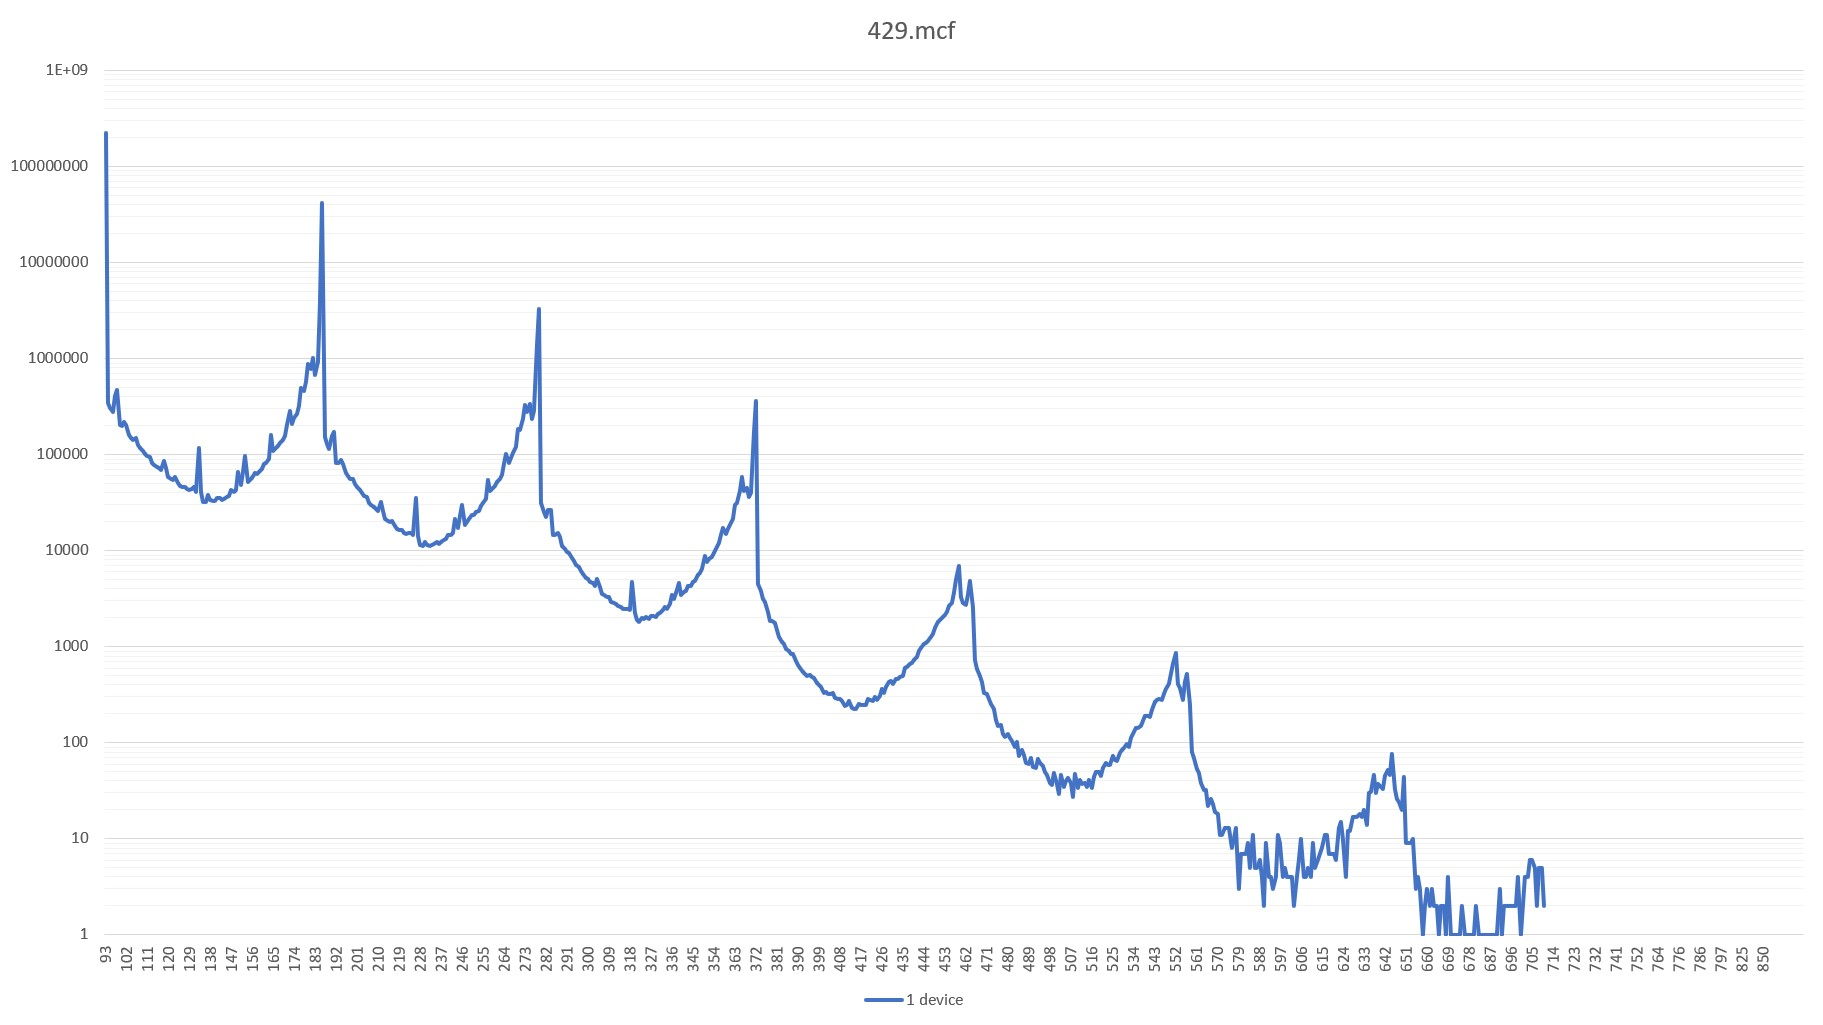
\includegraphics[width=1.0\linewidth]{figure/429-x.4-1.jpg}
    \caption{Access times using one device with four links, running 429.mcf.}
    \label{Memory-access-429-single}
\end{figure}

Adding more devices, and inherently placing data fruther from the host, will incurr greater latencies as seen in figure \ref{Memory-access-429}. However, it can be noted that the peaks all have about the same magnitude and the repeating pattern in between is reminescent of each other but with a few differences. These variations should be due to contention arising on the links when data to and from far-away devices tries to use the same links. It should also be noted that the contention looks different depending on distance, and while it mostly follows the access pattern from the optimal case it adds latencies at different places. Looking closer, in figure \ref{Memory-access-429-double}, where the access patterns of one and two devices respectively are put together, we can better distinguish between the patterns. We make sure to align the graphs in order to compensate for the hops distances. With the trend line for each setup we can see that there overall is some added latency with contention on the routing links. This gives rise to additional loss of performance. Interestingly, for this benchmark application, contention does not increase linearly with added number of devices, i.e. hops. Using four devices will increase the overall contention just slightly, while having six devices makes contention notably higher. The overall application performance still suffers from the added latency that multiple, long hops brings.

\begin{figure}[!h]
    \centering
    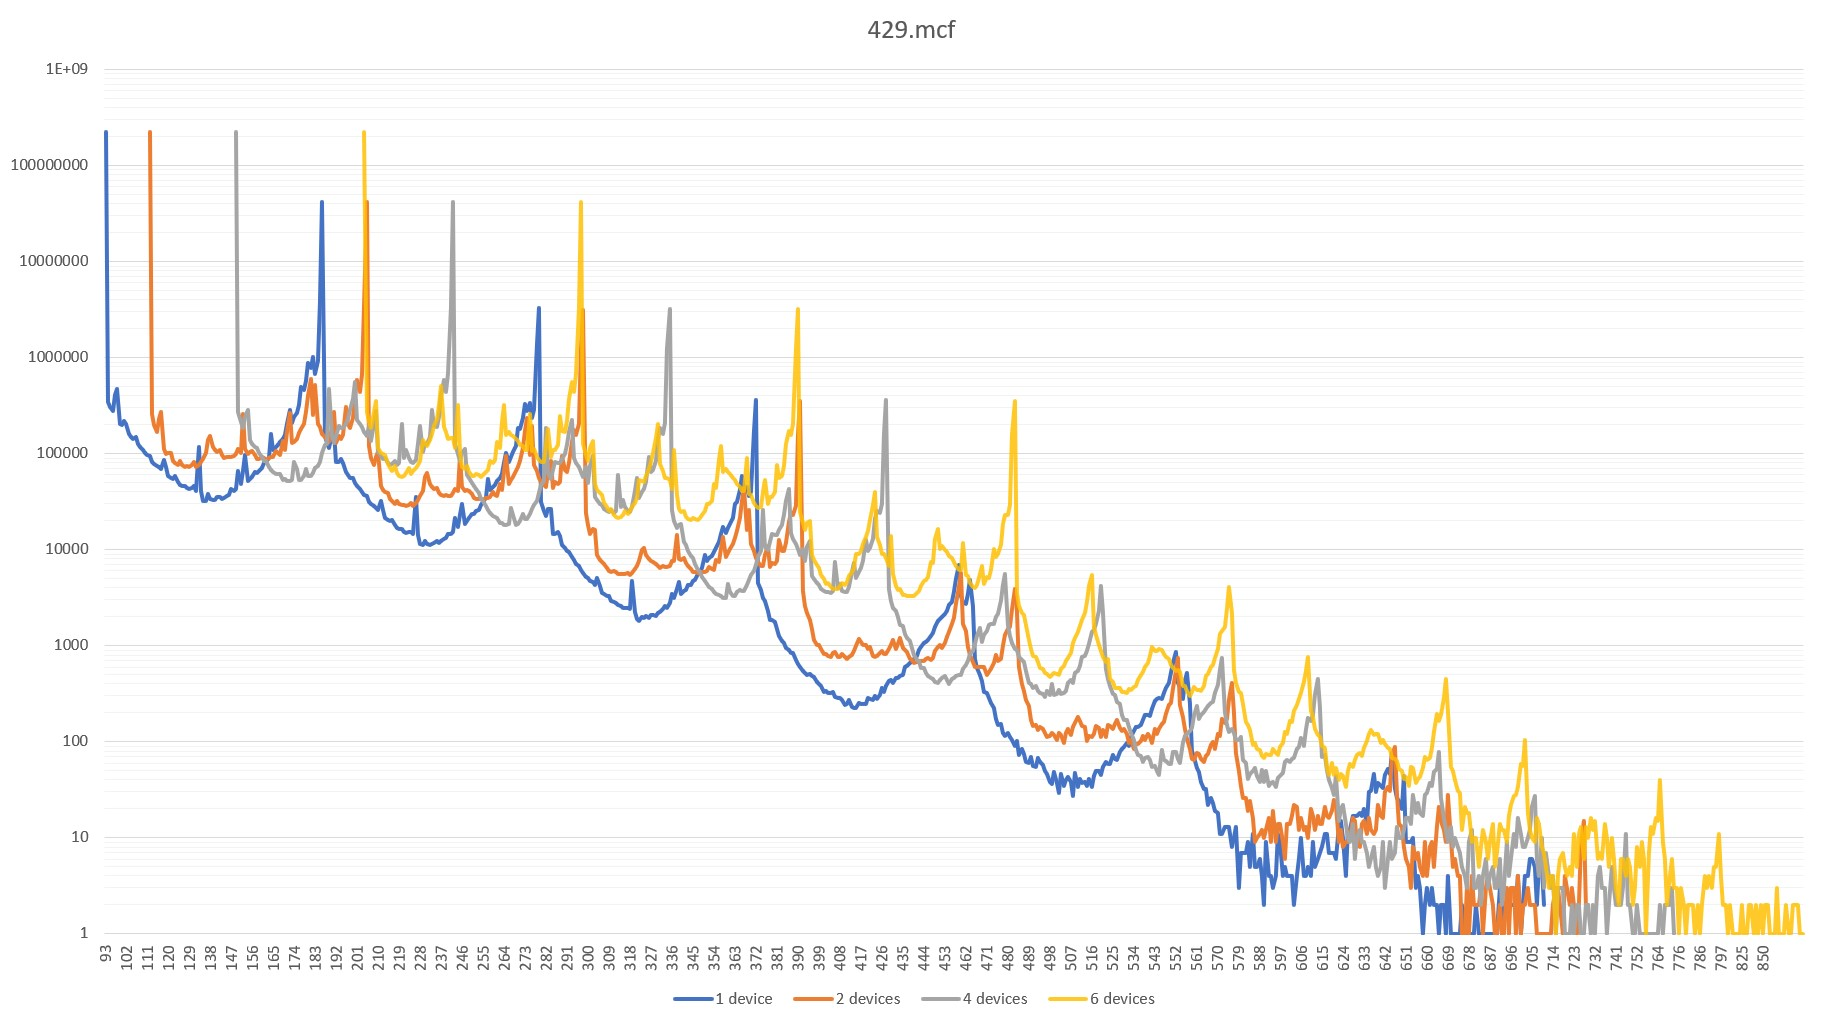
\includegraphics[width=1.0\linewidth]{figure/429-x.4.jpg}
    \caption{Comparing access times when using one, two, four and six devices.}
    \label{Memory-access-429}
\end{figure}

\begin{figure}[!h]
    \centering
    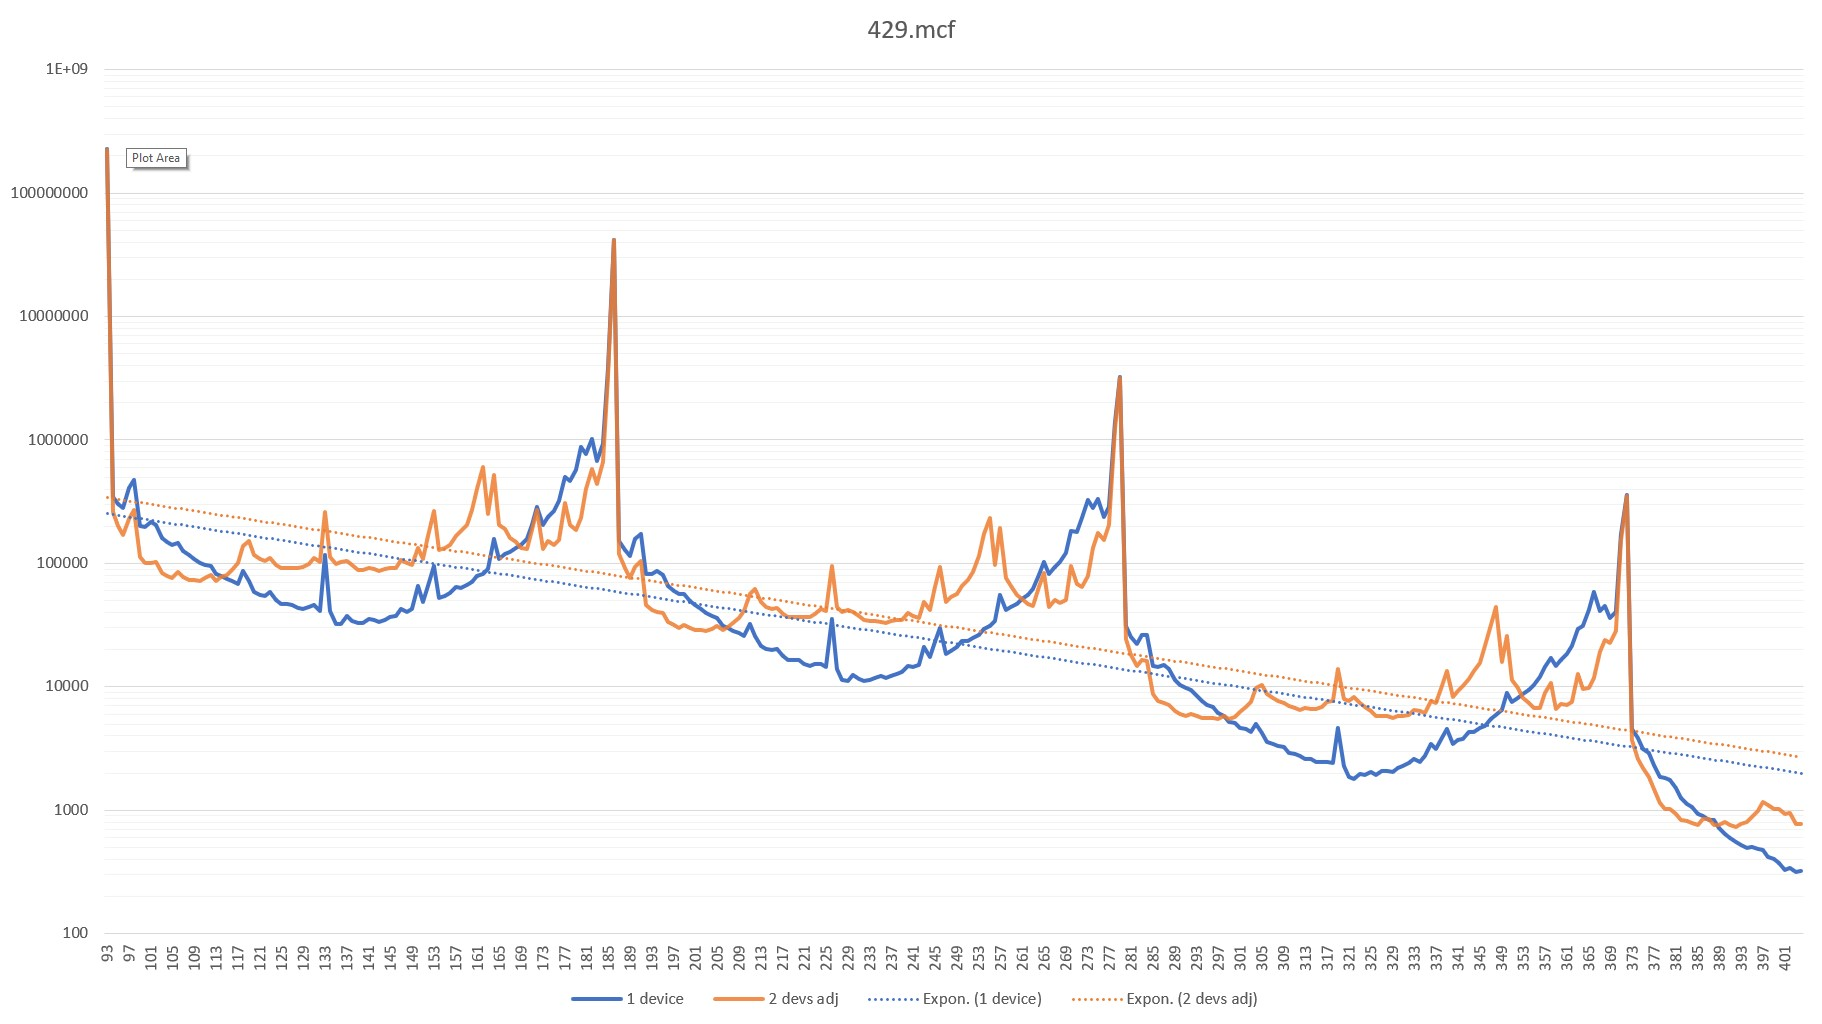
\includegraphics[width=1.0\linewidth]{figure/429-x.4-2.jpg}
    \caption{Part of the access patterns for one and two devices, where the latter has been adjusted to compensate for initial latency.}
    \label{Memory-access-429-double}
\end{figure}

Next we run using more links between the host and first device, as well as between individual cubes. Specifically, we now simulate using eight links instead of the previous four, of which four respectively two were usable (as explained in \ref{HMC-Sim}). This should to some extent alleviate the contention issue, but since the access scheme of the links is a simple round robin there might also be some added waiting time before data gets to the host. Running mcf using eight links and more than four devices turned out to take too long time (excess of 2 months run time) and those simulations were finally terminated. 

\begin{figure}[!h]
    \centering
    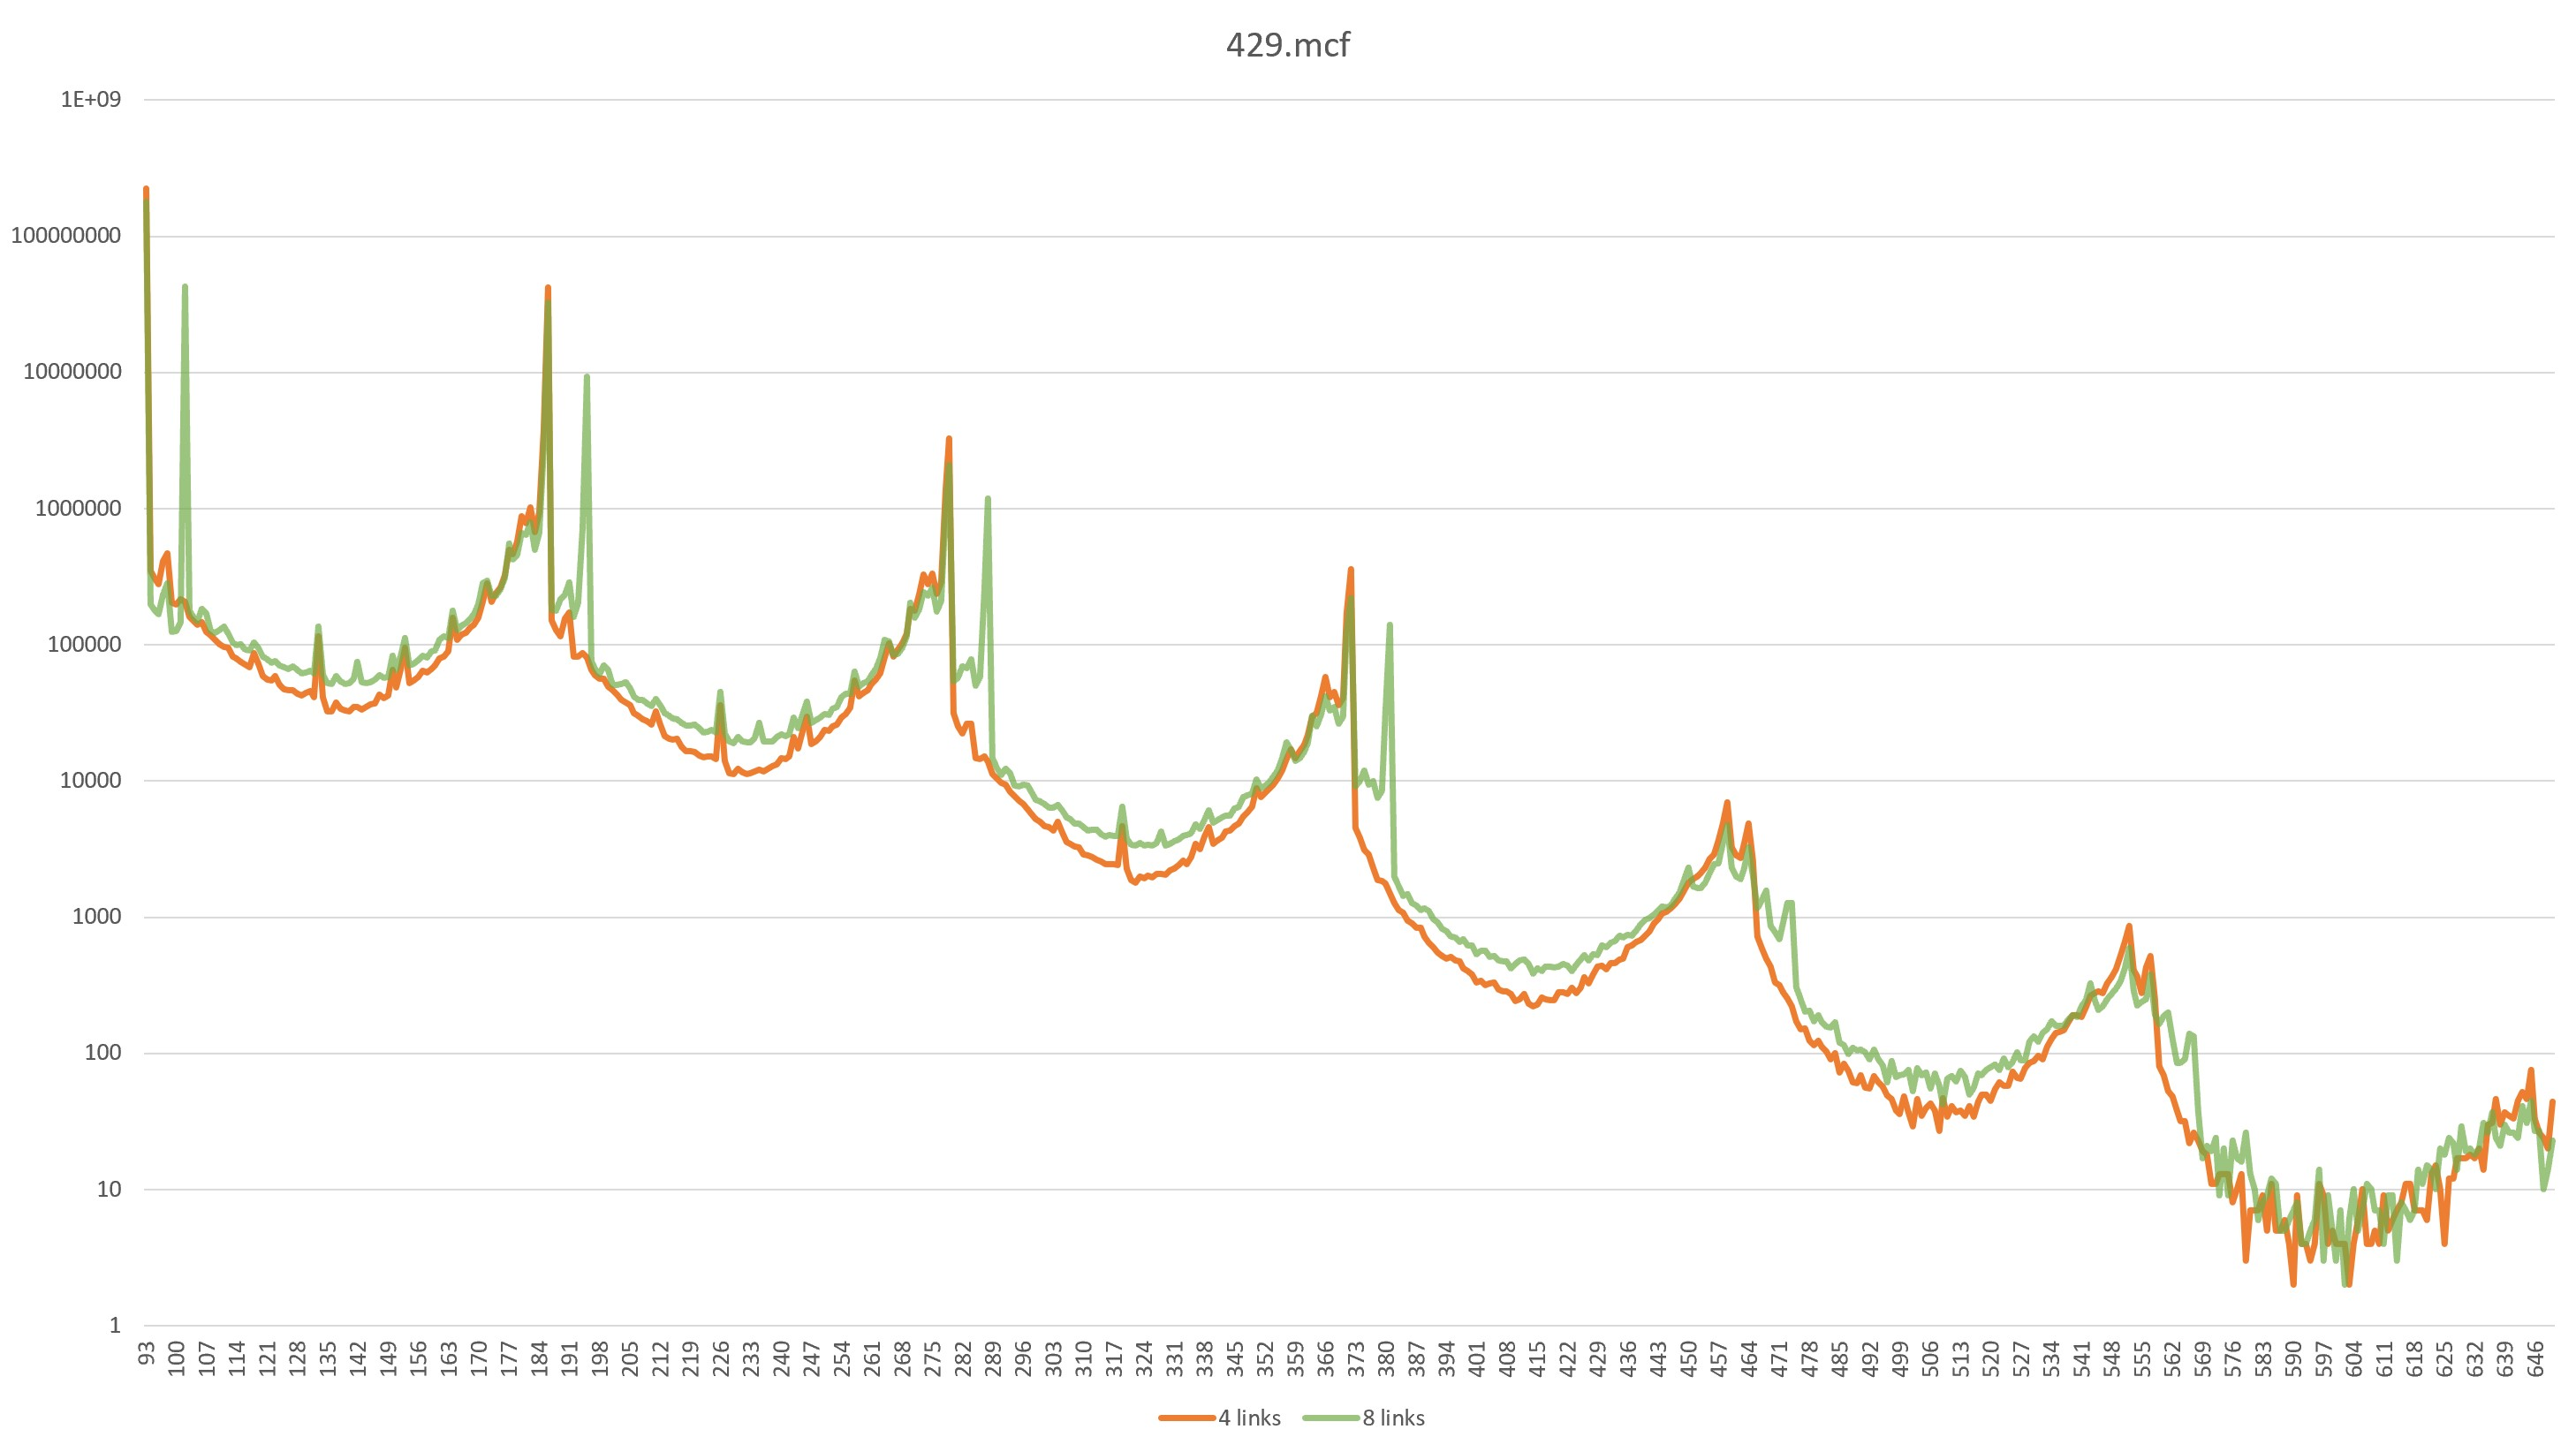
\includegraphics[width=1.0\linewidth]{figure/429-2.4-8.jpg}
    \caption{Part of the access patterns for one and two devices, where the latter has been adjusted to compensate for initial latency.}
    \label{Memory-access-429-link-compare}
\end{figure}

Running mcf using eight links produces some odd results. As can be seen in \ref{Memory-access-429-link-compare} the access pattern looks very much like using only four links, but there are new tailing spikes at 9 ns later. The second spike is a split of the otherwise always present 93 ns interval peak, where close to 20\% of all accesses are delayed with 9 ns. This could be due to how the host accesses each link with a round robin policy and that there is an additional wait introduced when the concurrency of multiple links cannot be utilised. By increasing bandwidth, through increased parallelism, we potentially worsen performance for this single application. However, when using two cubes, i.e. adding a hop, the patterns look almost identical. As such, the added latency of multiple links is cancelled out when having longer network traversal time.


% A first test was run with 429.mcf, which is arguably the most memory intense and latency sensitive benchmark out of the chose applications, just to see how the system's simulated memory would behave. This test was run using one active link and data allocated on the closest device. Figure \ref{Memory-access-behaviour} shows a graph over the number of times a specific access time, in ns, was reached for all simulated memory requests. The pattern seen is a more or a less repetitive form which reappears with 93 ns interval. The single link means that we only are connected directly to a single vault, and accesses to memory locations belonging to other vaults will have to be routed in the mesh network. However, since HMCSim probably does not perform a DRAM lookup -- which would incur a 93 ns latency, given our configuration -- for a request not belonging to the single vault, it is more likely that this pattern is due to HMC's Custom Memory Commands (CMC). A few such are implemented in HMCSim, e.g. for atomic access to multiple pages, and these will perform a new lookup for every requested page. The high amount of latency this adds is most likely due to HMC using a closed page policy, meaning that there will be no hits in the row buffer and even sequential data will have to fetched again.

% \begin{figure}[!h]
% \centering
% 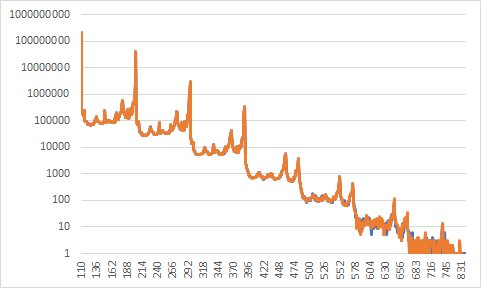
\includegraphics[width=0.75\linewidth]{figure/Testdata-4dev-4or1link-alloc0.png}
% \caption{Number of occurrences for different memory access times. }
% \label{Memory-access-behaviour}
% \end{figure}

\section{Summary}
Summarise the results without actually discussing the implications; leave that for the next part!